\begin{titlepage} 
    \begin{center}
         \begin{figure}[H]
            \centering
            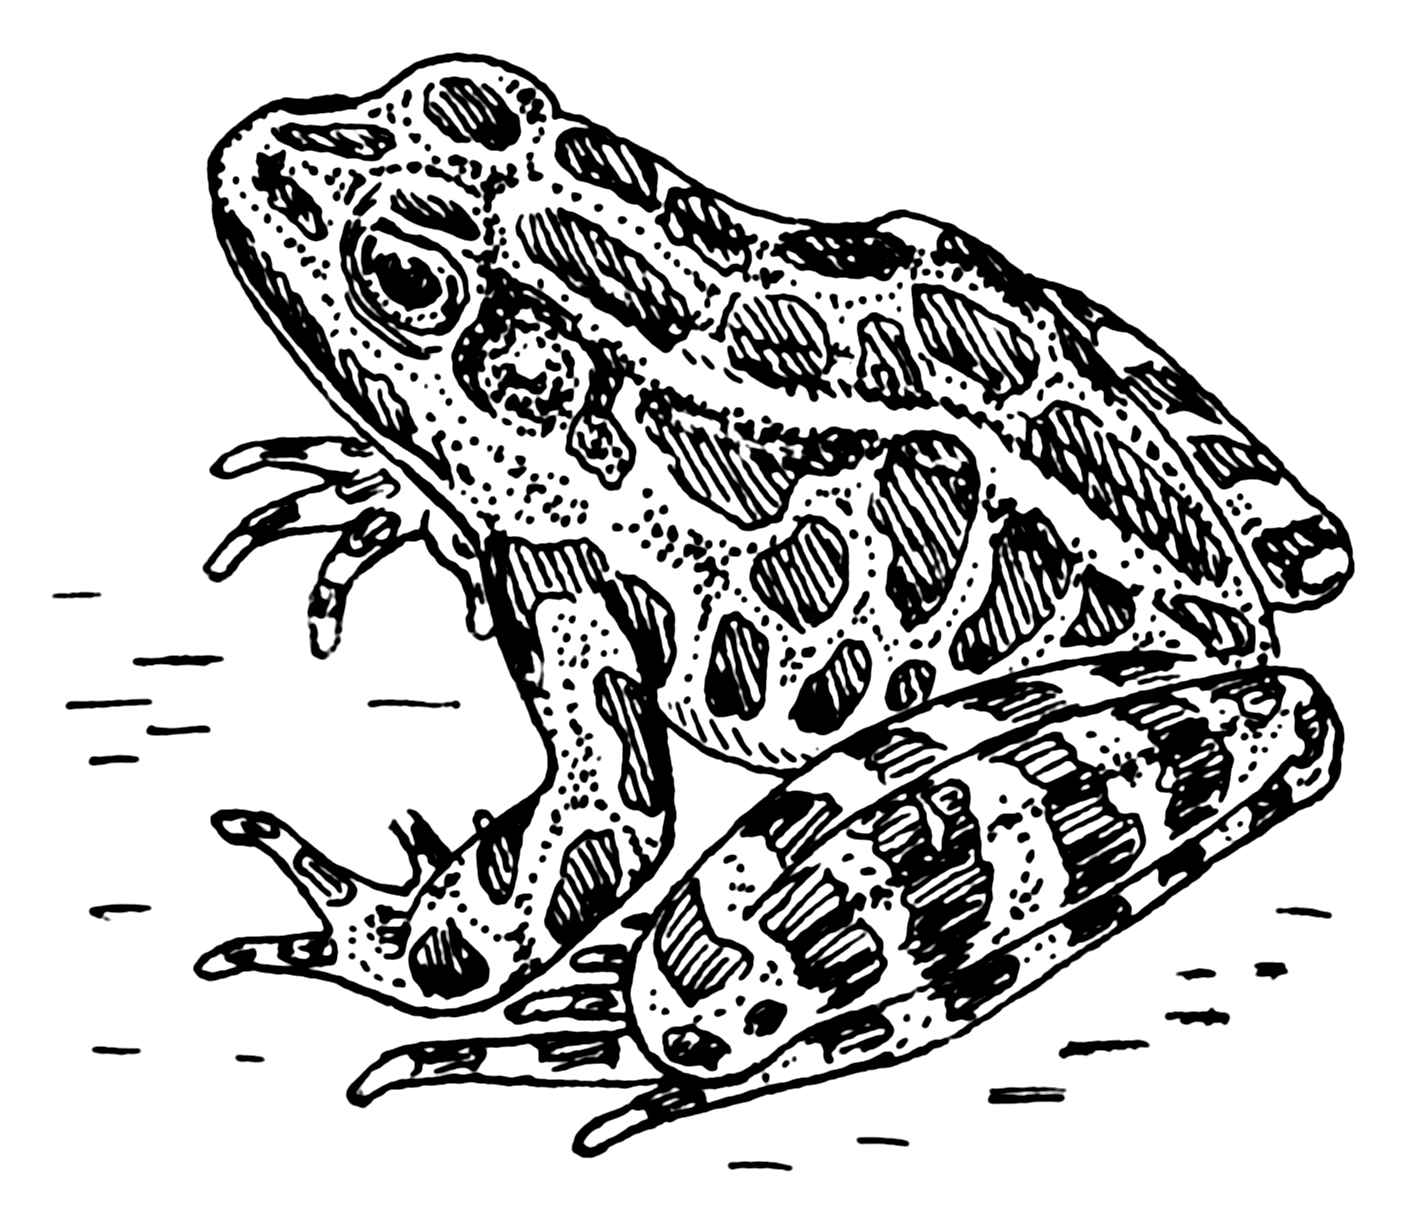
\includegraphics[scale=1]{img/Frog_(PSF).png}
           
        \end{figure}
        
        \Huge
        \textbf{\textsc{Egzamin licencjacki}}
        
        \vspace{0.5cm}
        \Large
        \textsc{Odpowiedzi na pytania} \\ 
        \line(1,0){330}

        \normalsize
        \textit{,,Nigdy nie rozumiałem po co ludzie czytają treści z obiektówki''}
        \vspace{1cm}

        \textit{\textsc{Autorzy}}\\
        \vspace{5mm}
  
        \textbf{\textsc{Dziurawy Ponton} \\ \textsc{Załatany Ponton} \\ \textsc{Puchaty Pompon} \\ \textsc{Zatopiony Ponton} \\ \textsc{Tonący Ponton}\\ \textsc{V} \\ \textsc{Nijaki Ponton} \\ \textsc{Pontus Euxinus}} \\
 
        \vfill

        Kraków \\
        Anno Domini 2024
    \end{center}
\end{titlepage}